\documentclass[tikz,border=3pt]{standalone}
\usetikzlibrary{arrows.meta}
\usepackage{newtxmath}
\begin{document}
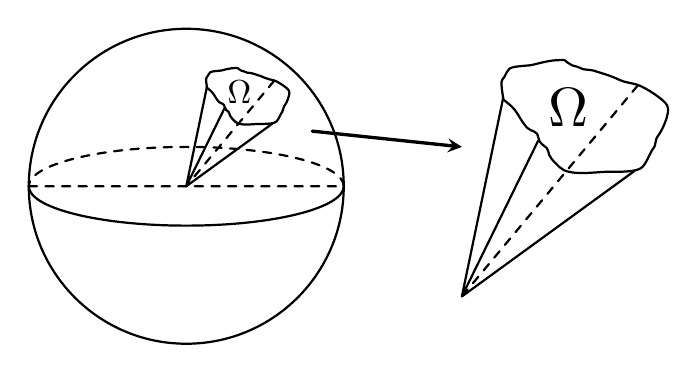
\begin{tikzpicture}[%
    thick,line join=round,line cap=round,
    pyramid/.pic={%
        \draw (0.486,1.009)
        .. controls (0.486,0.976) and (0.525,0.957) .. (0.539,0.943)
        .. controls (0.548,0.934) and (0.55,0.91) .. (0.555,0.898)
        .. controls (0.572,0.865) and (0.597,0.845) .. (0.621,0.821)
        .. controls (0.68,0.761) and (0.848,0.792) .. (0.928,0.792)
        .. controls (0.993,0.792) and (1.112,0.788) .. (1.145,0.821)
        .. controls (1.178,0.854) and (1.197,0.922) .. (1.218,0.943)
        .. controls (1.231,0.956) and (1.229,1.003) .. (1.243,1.017)
        .. controls (1.262,1.036) and (1.329,1.164) .. (1.304,1.213)
        .. controls (1.286,1.25) and (1.166,1.327) .. (1.116,1.344)
        .. controls (1.077,1.357) and (1.035,1.358) .. (0.997,1.377)
        .. controls (0.944,1.403) and (0.898,1.414) .. (0.838,1.434)
        .. controls (0.819,1.441) and (0.765,1.438) .. (0.752,1.451)
        .. controls (0.74,1.462) and (0.718,1.459) .. (0.703,1.467)
        .. controls (0.687,1.475) and (0.664,1.489) .. (0.654,1.5)
        .. controls (0.648,1.505) and (0.61,1.5) .. (0.6,1.5)
        .. controls (0.561,1.5) and (0.493,1.482) .. (0.449,1.471)
        .. controls (0.42,1.464) and (0.319,1.464) .. (0.302,1.446)
        .. controls (0.282,1.427) and (0.276,1.397) .. (0.257,1.377)
        .. controls (0.243,1.363) and (0.261,1.28) .. (0.261,1.266)
        .. controls (0.261,1.265) and (0.26,1.255) .. (0.261,1.254)
        .. controls (0.275,1.24) and (0.304,1.219) .. (0.318,1.205)
        .. controls (0.36,1.163) and (0.374,1.113) .. (0.416,1.07)
        .. controls (0.437,1.049) and (0.486,1.051) .. (0.486,1.009)
        .. controls (0.486,1.009) and (0.486,1.009) .. (0.486,1.009)
        -- cycle;
        \draw (0.263,1.264) -- (0,0) (0.485,0.99) -- (0,0)  (1.096,0.797) -- (0,0);
        \draw[dashed] (1.117,1.34)  -- (0,0);
        \node[scale=#1] at (0.675,1.2) {$\Omega$};
    }%
]
\draw circle [radius=2cm];
\draw[dashed] (-2,0) -- (2,0) arc[start angle=0,end angle=180,x radius=2cm,y radius=0.5cm];
\draw (-2,0) arc[start angle=180,end angle=360,x radius=2cm,y radius=0.5cm];
\pic {pyramid=1.2};
\pic[scale=2] at (3.5,-1.4) {pyramid=2};
\draw[-stealth,very thick] (1.6,0.7) -- (3.5,0.5);
\end{tikzpicture}
\end{document}